We now give every concept a second description, derived from the corpus alone.
A concept's \emph{usage vector} is the mean embedding of every passage in
which one of its aliases occurs as a whole word; \VecConcepts{} of the
\NConcepts{} concepts clear the threshold of \NoteMinSupport{} passages needed
for the mean to mean anything. Alongside it we keep the \emph{definition
vector} already used by the live query graph: the embedding of the concept's
label and the curator's gloss. The first is how the concept behaves in the
books; the second is what the curator says it is.

\paragraph{The subject matter has to be subtracted first.}
Every passage in this corpus is eighteenth-century moral philosophy, and that
shared subject is the largest single direction in the space. Left in, it
swamps everything: raw cosines between concept centroids run from 0.93 to
0.97, and pairs the map joins score \CosLinkedRaw{} against \CosUnlinkedRaw{}
for pairs it does not --- a real difference, but one three hundredths wide and
easy to mistake for noise. Subtracting the corpus mean removes the direction
every passage shares. The same comparison then reads \CosLinked{} against
\CosUnlinked{}, a gap ten times larger. Nothing about the data changed; the
common direction was simply removed from both sides. We report centred cosines
throughout, and note that any similar system which skips this step will find
that everything resembles everything.

\paragraph{The map is not arbitrary.}
Of \VecPairs{} concept pairs, \VecLinked{} are joined by at least one
assertion. Those pairs are markedly closer in the corpus than the rest
(\CosLinked{} against \CosUnlinked{}, Mann--Whitney $p<10^{-300}$), and
Figure~\ref{fig:vectors} shows the two distributions. A curator working from
the books, asserting relations by hand, produced something a distributional
model independently agrees with. The usage and definition descriptions agree
with each other more weakly ($\rho=\RhoUsageDef{}$), which is what one would
expect: a definition is written to distinguish a concept from its neighbours,
while usage records that they appear in the same paragraphs.

\begin{figure}[t]
  \centering
  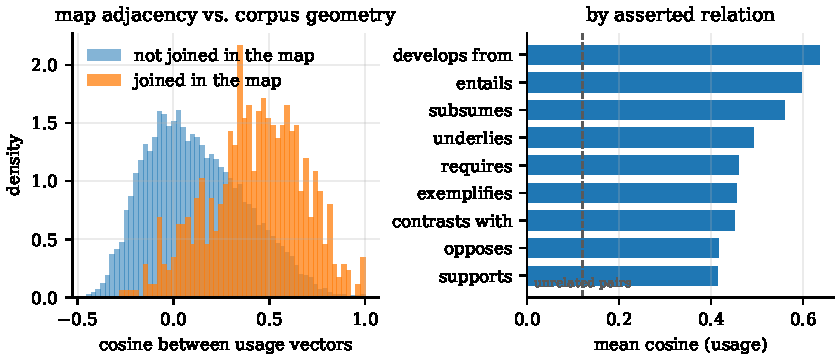
\includegraphics[width=\linewidth]{map_vs_vectors.pdf}
  \caption{Left: centred cosine between concept usage vectors, for pairs the
           map joins and pairs it does not. Right: mean cosine by the kind of
           relation asserted, against the unlinked baseline (dashed). The
           relations that order concepts hierarchically sit highest; the
           relations that set concepts against each other sit at the bottom,
           level with \rel{supports}.}
  \label{fig:vectors}
\end{figure}

\paragraph{The geometry cannot hear a negation.}
The right panel of Figure~\ref{fig:vectors} is the substantive result. Sort
the relation types by how close their pairs sit, and the order is
\rel{develops\_from} (\CosDevelopsFrom{}), \rel{entails} (\CosEntails{}),
\rel{subsumes} (\CosSubsumes{}), \rel{underlies} (\CosUnderlies{}),
\rel{requires} (\CosRequires{}), then \rel{contrasts\_with}
(\CosContrastsWith{}), \rel{opposes} (\CosOpposes{}) and \rel{supports}
(\CosSupports{}).

Two things follow. The first is that relations which arrange concepts in a
hierarchy --- one develops from another, entails it, subsumes it --- are the
ones the vector space reproduces most strongly, which makes sense: a concept
that subsumes another is discussed wherever the other is.

The second is sharper. \rel{opposes} scores \CosOpposes{} and \rel{supports}
scores \CosSupports{}. They are indistinguishable. A pair of concepts the
curator marked as standing against each other sits exactly as close, in the
corpus, as a pair marked as holding each other up --- and both sit some three
and a half standard deviations above the unlinked baseline. The geometry
registers that two concepts belong to the same argument; it has no access
whatever to which side of it they are on. This is the antonymy problem
\citep{mohammad2013,nguyen2016} arriving in a corpus where it does real damage,
because the century's central disputes are precisely oppositions: self-love
against benevolence, interest against duty, reason against sentiment. A
semantic search for evidence that an author held a position will return, with
equal confidence, the passage in which a rival denies it. The system's
verification tool, which re-reads the retrieved page before a claim is made,
exists for this reason; here is the measurement that justifies it.

\paragraph{Where the vectors correct the map.}
The pairs that sit closest in the corpus while carrying no assertion at all
are almost entirely a single kind of thing: near-duplicate concepts.
\concept{Lipsius Citation} and \concept{Seneca} have a cosine of 1.000,
meaning their aliases select identical passages. \concept{Seneca} and
\concept{Seneca Reference}, \concept{Fitness} and \concept{Moral Fitness},
\concept{Atheism} and \concept{Virtue and Atheism}, \concept{Evil} and
\concept{Origin of Evil}, \concept{Sacrament} and \concept{Sacramental
Remembrance} --- all above 0.98, none joined by an edge. The vector space is
acting here as an auditor of the ontology, and what it reports is that the map
contains a dozen concepts that are variants of another concept rather than
concepts in their own right. This is the single most directly actionable
result in the paper: these pairs are candidates for merging.

\paragraph{Where the map outruns the corpus.}
The reverse list --- pairs the map joins that the corpus places furthest apart
--- reads differently. \concept{Moral Fitness} \rel{supports}
\concept{Trinity} at $-0.26$, \concept{Sacrament} \rel{requires}
\concept{Virtue} at $-0.23$, \concept{Reason} \rel{requires}
\concept{Sacrament} at $-0.20$. These are not obviously wrong as claims about
the period; they are claims whose two halves live in different books, one
theological and one ethical, and which therefore have no shared context for a
distributional method to find. They are the assertions a reader of the whole
library can make and a model trained on passage co-occurrence cannot. Whether
they are insights or overreach is not something the geometry can settle, and
we do not pretend otherwise --- but they are exactly the list a curator should
be handed when asked to defend the map.
